\cleardoublepage
\chapter{相关工作}

\section{面向物联网时序数据的集中式存储系统}
在物联网的传统存储系统中,中心化存储系统通常以其强大的数据处理能力和集中的数据控制而受到青睐。
这种存储方式依托于中心节点的强大计算和存储能力,处理来自众多物联网设备的数据。
集中式存储简化了数据管理流程,便于实现数据的统一备份和恢复,同时易于实施安全控制措施,如访问权限管理和数据加密。

AWS IoT~\cite{aws}是亚马逊云服务(Amazon Web Services)提供的一个集中式云平台,专门设计用于支持和简化物联网设备的连接、管理和数据收集工作。
作为一个集中式的解决方案,AWS IoT提供了一个中心化的服务,允许来自全球各地的设备安全地将数据流传输到亚马逊的云基础设施中。
通过集中式架构,AWS IoT能够为设备数据提供一个统一的接入点,使得数据的管理和监控变得更加高效。
这种集中式存储方式意味着所有的设备数据都汇聚到AWS的数据中心,由AWS进行集中管理和处理。

TDengine~\cite{tdengine}是一个为处理时序数据而特别设计的高性能、分布式、支持SQL的集中式数据库系统。
它以其卓越的性能和对时间序列数据的优化而受到关注,能够处理高吞吐量的数据写入和查询。
为了减少每个数据存储分片之间的通信开销,TDengine将分片存储在中心节点上,
此外,TDengine支持多种编程语言的API,包括C、Python和Java,这使得它可以轻松地集成到各种应用程序中。

TinyDB~\cite{madden2005tinydb}是一个为传感器网络设计的查询处理系统,它通过一种称为获取式查询处理的方法来优化传感器网络中的时序数据采集和查询处理。
TinyDB将数据集中存储在中心节点,以此来减少数据传输和处理的开销,同时提供了对数据的高效查询和分析功能。

然而,尽管中心化存储系统在管理和控制方面具有优势,但它们也存在着一些不可忽视的问题。
最主要的问题之一是单点故障风险,即如果中心存储节点发生故障,整个系统的数据存储功能可能会受到严重影响,甚至导致数据的不可用或丢失。
恶意行为者只需针对中心节点发起攻击,就有可能破坏整个系统的稳定性,甚至盗取存储的数据。
此外,随着物联网设备的激增和数据量的爆炸式增长,中心化存储系统可能会遇到扩展性瓶颈,处理和存储大量数据的需求可能会导致中心节点的性能瓶颈。

随着技术的发展,特别是区块链和分布式存储技术的进步,越来越多的解决方案开始倾向于去中心化,以提高系统的可靠性和安全性。
中心化存储系统的局限性促使研究者和开发者寻求更为稳健的存储解决方案,以应对日益增长的数据存储需求。

\section{面向物联网时序数据的分布式存储系统}
与集中式存储相比,分布式数据库将数据分散存储在多个节点或数据中心中,这使系统本身就具备了抗单点故障的能力。
即使某个节点或数据中心发生故障,系统仍然可以继续运行并提供服务,从而保障了数据的可靠性和稳定性。
因此,随着对数据安全性、可用性和性能要求的不断提高,分布式数据库作为一种能够克服集中式存储固有弱点的解决方案,逐渐成为了当今大数据时代的主流选择。

Apache Cassandra~\cite{lakshman2010cassandra}作为一个分布式结构化键值存储系统,借鉴了Dynamo~\cite{decandia2007dynamo}的分布式系统技术和Google BigTable~\cite{chang2008bigtable}的数据模型优势,通过特殊的数据分发策略确保数据存储的高可用性和容错性。
其灵活的数据模型和分布式特性使得它适用于需要横向扩展和高性能的应用场景。

Spanner~\cite{corbett2013spanner}是谷歌开发的全球分布式数据库。
它通过TrueTime API~\cite{cervin2016truetime}提供的时间戳服务实现全球性一致性和高可用性,并结合关系型数据库的ACID属性和分布式数据库的横向扩展,适用于需要高度一致性和水平扩展的工业应用场景。

\begin{figure}[t]
    \centering
    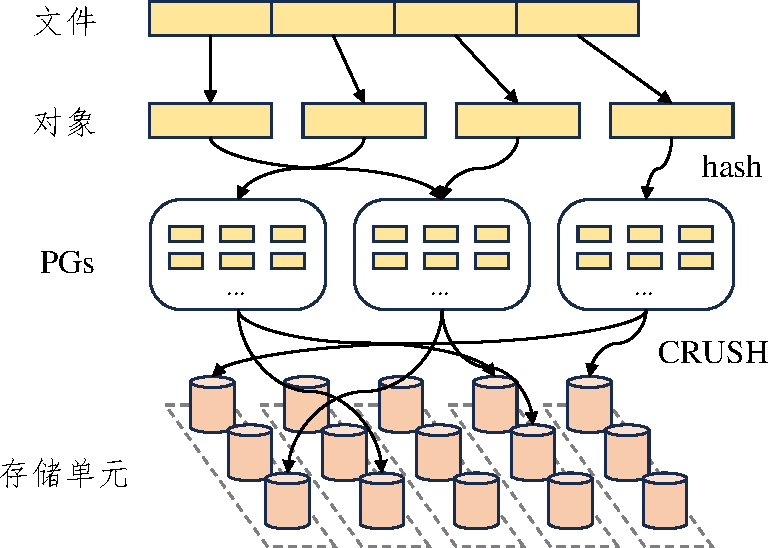
\includegraphics[width=0.7\linewidth]{figures/timechain/ceph.pdf}
    \caption{Ceph存储流程}
    \label{fig:ceph}
\end{figure}

Ceph~\cite{weil2006ceph}作为一个开源的分布式存储系统,提供对象存储、块存储等功能。
为了平衡各存储节点的压力,它提出了可扩展哈希下的受控副本(Controlled Replication Under Scalable Hashing,CRUSH)算法,用于数据的分布式存储和数据冗余备份。
如\autoref{fig:ceph}所示,对于需要被存储的文件而言,Ceph会首先将文件划分成多个独立的对象,然后Ceph将对象根据哈希分成若干放置组(Placement Group,PG)。
随后,CRUSH算法结合地理位置信息将PG映射到存储集群中的存储节点,实现数据的均衡分布和高效访问。
这种分布式的数据分布方式使Ceph系统具有高度的可扩展性和容错性,即使在节点故障或网络分区的情况下,系统仍能保持数据的可靠性和可用性。

CockroachDB~\cite{taft2020cockroachdb}在Spanner的基础上,通过设计结合地理信息的复制和自动恢复机制来实现高容错性。
它将数据分布在不同的地理位置或数据中心,确保数据的冗余备份分布在不同的地理区域。
这种地理信息复制策略使得即使某个地理区域发生故障,数据仍然可以从其他地理位置的备份节点进行恢复。

然而,这些分布式存储系统仍然存在着单点故障和高存储成本的问题。
这是因为即使数据存储在不同位置,数据的管理仍然是中心化的。
在这些存储系统中,公司有可能在数据拥有者不知情的情况下轻松篡改数据,直接危及数据的完整性和安全性。
这些缺陷限制了这些系统在处理物联网数据激增和复杂协作需求方面的灵活性和效率,同时也使得数据的安全性和可靠性备受质疑。
因此,解决这些问题对于推动分布式存储系统在未来应用中获得广泛应用至关重要。

\section{基于区块链的存储系统}
区块链技术的出现为分布式存储系统的安全性和可靠性提供了新的解决方案。
区块链存储系统是一种基于区块链技术的分布式存储解决方案,其核心概念是将数据分布式存储在网络中的多个节点上,并使用区块链作为数据的验证和记录机制。
在区块链存储系统中,数据被分割成块,并以链式连接的方式进行存储,每个数据块包含了前一个块的哈希值,从而构成了不可篡改的数据记录链。
这种数据结构使得数据的完整性和安全性得到了极大的保障,任何尝试篡改数据的行为都会被系统所记录和拒绝。
区块链存储系统的去中心化特性意味着数据的管理不再依赖于单一实体,而是由网络中的多个节点共同维护和验证。
这种设计使得数据拥有者可以更加信任系统,因为数据的安全性和可靠性不再受限于单一实体的控制。

根据数据的存储位置,区块链存储系统可以分为链上存储和链下存储。

\subsection{面向交易数据的链上存储}
目前,许多链上存储的研究都集中在链上数据存储的性能上,包括优化链上存储的查询性能和减少链上存储负担等。

\begin{figure}[t]
    \centering
    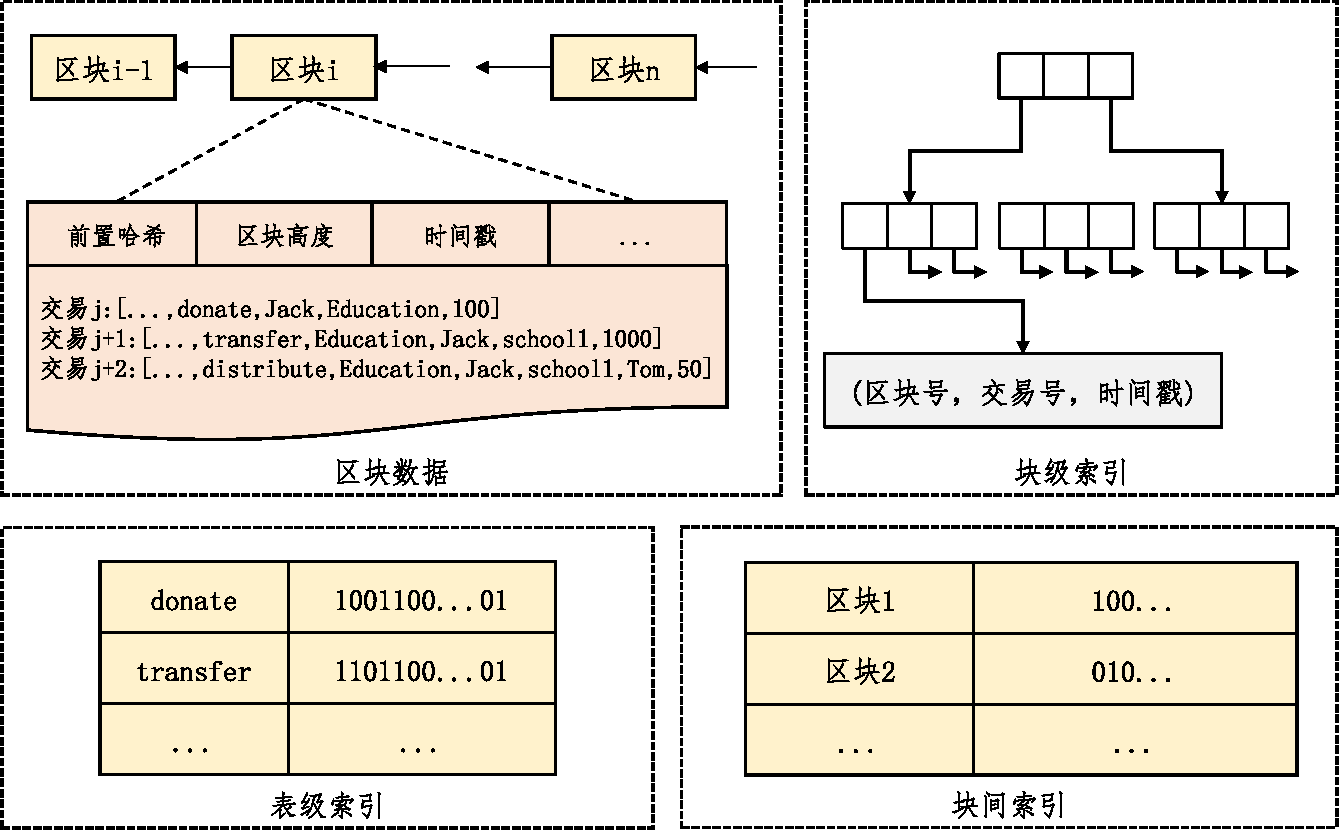
\includegraphics[width=1\linewidth]{figures/timechain/sebdb.pdf}
    \caption{SEBDB数据结构}
    \label{fig:sebdb}
\end{figure}

部分工作关注于增强链上存储的查询支持。
由于区块链的交易数据都是以日志的形式存储在区块链上,无法提供类似关系型数据库的高效查找。
因此,一些工作提出了在区块链上建立索引的方法,以支持对区块链数据的高效查询。
SEBDB~\cite{zhu2019sebdb}将关系数据语义添加到区块链信息中,将每个事务视为预定义表中的元组,并使用类似SQL的语言作为通用接口,以支持方便的应用程序开发。
如\autoref{fig:sebdb}所示,SEBDB使用B+树建立了块级索引,将真实的数据组织成B+树,以支持类SQL查询。
SEBDB也建立了表级索引和块间索引,便于快速定位区块位置。
MSTDB~\cite{zhou2022mstdb}则建立了基于语义的索引结构默克尔语义树(Merkle Semantic Trie,MST),以此支持基于语义的多关键字查询、Top-K查询、范围查询和跨链查询。
MSTDB也使用索引压缩和布隆过滤的方式减少索引的存储开销,提高了查询性能。

\begin{figure}[t]
    \centering
    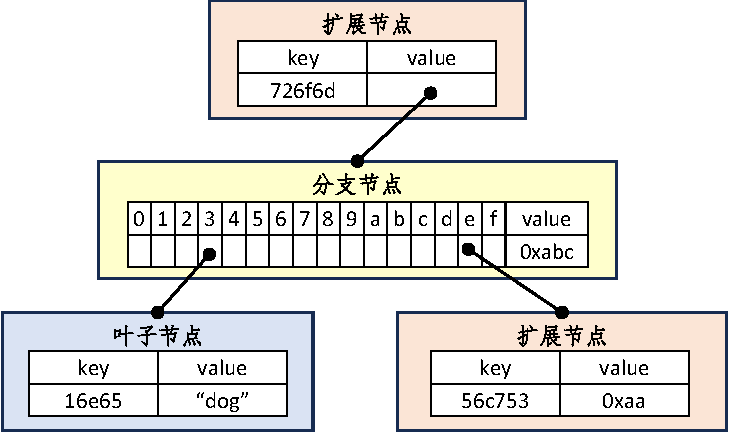
\includegraphics[width=0.75\textwidth]{figures/timechain/mpt.pdf}
    \caption{默克尔帕特里夏树结构}
    \label{fig:mpt}
\end{figure}

也有部分工作优化了区块上的索引和认证机制,以提高区块链状态的查询速度。
默克尔帕特里夏树(Merkle Patricia Tree,MPT)是以太坊区块链中底层的数据结构,用于存储账户状态和交易信息。
如\autoref{fig:mpt}所示,MPT由三种类型的节点构成:叶子节点、扩展节点和分支节点。
叶子节点包含实际的键值对,扩展节点包含指向其他节点的哈希值的键值对。
分支节点包含多个可能的子节点路径,该节点使用十六进制进行编码分支。
每个节点都用哈希值确保节点数据的完整性。
针对MPT的磁盘访问开销,LVMT~\cite{li2023lvmt}设计了认证多点评估树(Authenticated Multipoint Evaluation Tree,AMT)在常数时间内更新完整性证明,并且采用多层设计来支持无限的键值对。
LVMT通过层级设计增强键值对可扩展性,通过存储版本号替代哈希的方式避免了昂贵的椭圆曲线乘法运算。
针对MPT的索引重复存储开销,COLE~\cite{zhang2024cole}引入新兴的学习索引技术优化了区块链的存储索引结构。
具体而言,COLE遵循基于列的数据库设计来连续存储每个状态的历史值,这些历史值由学习模型索引,以促进高效的数据检索和出处查询。
COLE将数据按状态地址连续存储,通过学习索引模型减少存储索引开销;并针对区块链的存储磁盘特性引入了LSM树,以支持高效的读写性能。

部分工作关注链上存储的性能优化。
FalconDB~\cite{peng2020falcondb}和Chen等人提出的仲裁模型~\cite{chen2022blockchain}都关注区块链节点之间数据交互的效率。
为了减轻区块链账本数据存储的负担,Rapidchain~\cite{zamani2018rapidchain}、SlimChain~\cite{xu2021slimchain}和GriDB~\cite{hong2023gridb}将账本的数据分配给其他分片存储,以减轻存储压力。

在大规模数据生成迅速的物联网场景中,上述解决方案存在两方面的挑战:

\begin{itemize}
    \item[$\bullet$] 首先,这些解决方案会给区块链带来额外的空间存储负担。
    由于物联网设备在短时间内生成的数据量庞大,将这些数据全部存储在区块链上可能会导致链的存储需求急剧增加,进而增加系统的复杂性和成本。
    \item[$\bullet$] 其次,这些方案可能导致数据隐私泄露的风险增加,因为在区块链上存储的数据通常是不可篡改和公开可见的,这会导致物联网的数据泄露。
\end{itemize}

综上所述,在数据密度低、生成速度快的物联网场景下直接使用传统的链上存储方案,会产生较大的开销和风险。
物联网场景需要更加注重数据存储效率和隐私保护,因此需要针对这些特殊需求设计更为灵活和高效的数据管理方案。

\subsection{面向文件数据的链下存储}

\begin{figure}[t]
    \centering
	\begin{minipage}{0.45\linewidth}
        \centering
        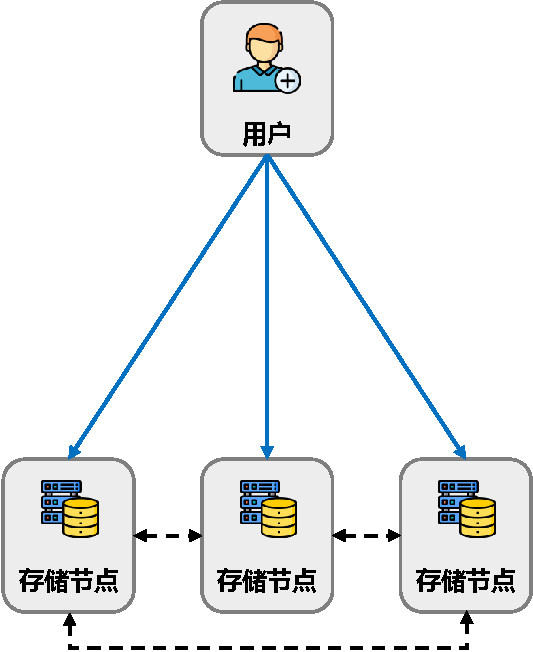
\includegraphics[width=1\textwidth]{figures/timechain/filedes.pdf}
        \caption{去中心化存储系统}
        \label{fig:filedes}
	\end{minipage}
	\quad
	\begin{minipage}{0.45\linewidth}
        \centering
        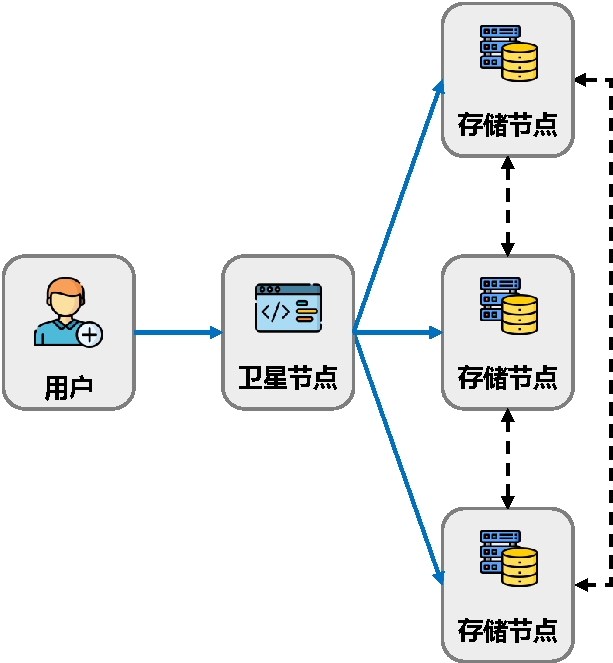
\includegraphics[width=1\textwidth]{figures/timechain/storj.pdf}
        \caption{半去中心化存储系统}
        \label{fig:storj}
    \end{minipage}
\end{figure}

基于区块链的文件系统因其较少的开销而备受广泛研究和关注。
这些系统将文件本身存储在链下,规避了原始数据直接存储在链上带来的巨大开销,并通过在区块链上记录文件的哈希值和验证信息来确保文件的完整性和安全性。
由于区块链的不可篡改性,用户可以方便地验证文件的来源和完整性,防止数据篡改和丢失。
相较于传统的中心化存储系统,基于区块链的文件系统通常不需要中心化的服务器和高昂的维护成本,从而降低了整体的运营成本。

Storj~\cite{storj2018storj}和Sia~\cite{vorick2014sia}是两个典型的半去中心化的文件存储系统。
如\autoref{fig:storj}所示,在半去中心化网络中,除了存储节点,也存在一组卫星节点。
这些卫星节点通过运行特定的智能合约来处理用户的请求,例如选择存储节点、进行文件切分、索引文件等。
他们也为每个文件建立默克尔树以确保文件的完整性。

FileCoin~\cite{bauer2022filecoin}是建立在IPFS~\cite{benet2014ipfs}上的去中心化文件存储系统。
IPFS是一种点对点的分布式文件系统,它通过内容寻址来存储和共享文件,使得文件在没有单点故障的分布式网络上可用。
通过激励机制鼓励用户提供存储服务,FileCoin利用区块链技术确保了文件的完整性和可靠性,同时为用户提供了一种去中心化的存储解决方案。
如\autoref{fig:filedes}所示,在FileCoin中,节点可以通过提供存储空间来获取FileCoin代币奖励,从而构建一个分布式的文件存储网络。
对于这个完全去中心化的系统而言,所有存储节点之间都是平等的,每个节点将参与到用户的请求处理过程中。
这种模式不仅激励了更多的存储资源加入网络,还提高了数据的持久性和可访问性,因为文件被分散存储在全球各地的节点上,减少了中心化存储的风险。
为了确保文件的完整性,FileCoin为每个文件建立默克尔树,通过分散存储文件块来提高可靠性和安全性,从而降低了数据丢失的风险。
用户可以通过这些系统安全地存储和共享文件,同时保持数据的隐私和安全性。

FileDES~\cite{xu2024filedes}专注于数据的加密存储,借助零知识证明等技术来保护数据的安全性。
通过加密存储数据,FileDES可以确保用户的数据在存储和传输过程中不会被泄露或篡改。
这种方法为用户提供了更高级别的数据安全保障,尤其适用于对数据隐私和安全性要求较高的场景。

然而,尽管这些方法在确保文件完整性和安全性方面表现出色,它们并不适用于高效存储物联网数据的存储。
这是因为物联网数据通常具有较低的价值密度,而将单个数据以文件形式存储在区块链文件系统中,将导致极高的成本。
物联网数据的特点决定了需要更为轻量级和高效的数据存储方案,以更好地应对数据生成量大、频繁性高的特点,同时降低存储和处理成本。
因此,对于物联网大规模数据存储的需求,寻找轻量、高效、可信的数据解决方案是一个挑战。

\begin{table}
    \centering
    \caption{物联网存储系统比较}
    \begin{tabular}{|l|c|c|c|c|} 
    \hline
     & 去中心化 & 链上/链下 & 可扩展性 & 数据类型 \\ 
    \hline
    AWS IoT~\cite{aws} & \emptycirc & - & \fullcirc & 传感器数据 \\ 
    \hline
    TDengine~\cite{tdengine} & \emptycirc & - & \fullcirc & 传感器数据 \\ 
    \hline
    TinyDB~\cite{madden2005tinydb} & \emptycirc & - & \fullcirc & 传感器数据 \\ 
    \hline
    Spanner\cite{corbett2013spanner} & \emptycirc & - & \fullcirc & 传感器数据 \\ 
    \hline
    CockroachDB\cite{taft2020cockroachdb} & \emptycirc & - & \fullcirc & 传感器数据 \\ 
    \hline
    SEBDB\cite{zhu2019sebdb} & \fullcirc & 链上 & \emptycirc & 传感器数据 \\ 
    \hline
    MSTDB\cite{zhou2022mstdb} & \fullcirc & 链上 & \emptycirc & 传感器数据 \\ 
    \hline
    Filecoin\cite{bauer2022filecoin} & \fullcirc & 链下 & \fullcirc & 文件 \\ 
    \hline
    Storj\cite{storj2018storj} & \fullcirc & 链下 & \fullcirc & 文件 \\ 
    \hline
    FileDES\cite{xu2024filedes} & \fullcirc & 链下 & \fullcirc & 文件 \\ 
    \hline
    TimeChain & \fullcirc & 链下 & \fullcirc & 传感器数据 \\
    \hline
    \end{tabular}
\end{table}

\section{本章小结}
本章广泛探讨了面向物联网的分布式存储系统和基于区块链的存储系统的相关研究工作。
本章分析了集中式数据存储解决方案的局限性,特别是它们在面对单点故障时的脆弱性,以及分布式数据库如何通过在多个节点间分散存储数据来提高数据的可靠性和稳定性。
其次,详细讨论了Apache Cassandra、Spanner、Ceph和CockroachDB等分布式存储系统,它们通过不同的技术手段实现了数据的高可用性和容错性。
然而,这些系统仍然存在单点故障的风险,并且由于数据管理的中心化,数据的完整性和安全性仍然受到威胁。

进一步地,本章探讨了基于区块链的存储系统,它们通过将数据分布式存储在多个节点上,并利用区块链作为数据验证和记录的机制,提供了一种新的数据存储解决方案。
本章分析了链上存储和链下存储两种方法,以及它们在提高数据存储性能和确保数据完整性方面的研究进展。
尽管这些基于区块链的存储系统在确保数据完整性和安全性方面具有优势,但它们在处理大规模、低价值密度的物联网数据时面临效率和成本的挑战。

综上所述,现有的分布式存储系统和基于区块链的存储系统虽然在某些方面取得了进展,但它们在满足物联网数据存储需求方面仍存在不足。
这些挑战包括处理大规模数据的效率、数据存储的成本以及数据隐私保护的需求。
因此,开发一种轻量级、高效且可信的数据存储解决方案对于物联网领域来说是一个重要的研究方向。
TimeChain正是在这样的背景下应运而生,旨在结合区块链技术的优势,解决物联网时序数据存储中的关键问题。
